%{{{-----------------------------------Basics----------------------------------%

%document class definition
\documentclass[
    11pt,
    a4paper,
    oneside,
    headinlcude, footinclude,
    twoside,
]{report}


%essential packages
\renewcommand*\rmdefault{ppl}
\usepackage[top=2.5cm,bottom=2.5cm,left=3cm,right=3cm]{geometry}
\usepackage[english]{babel} \usepackage[T1]{fontenc} \usepackage[utf8]{inputenc} \usepackage{xcolor} \usepackage{amssymb}


%additional packages
\usepackage{amssymb}
\usepackage{amsmath}
\usepackage[framemethod=Tikz]{mdframed}
\usepackage{tikz}
\usepackage{enumerate}
\usepackage{pgf,tikz,pgfplots} % for the transfer from geogebra to tikz
\usepackage{mathrsfs}% for the transfer from geogebra to tikz
\usepackage{graphicx}
\usepackage[makeroom]{cancel}
\usepackage{fancyhdr}
\usepackage{makecell} %to have thick hlines in the front page
\usepackage{tabularx}

%}}}

%{{{-----------------------------------Macros----------------------------------%

\newcommand{\myImplies}[0]{\rightarrow}

\newcommand{\powerset}[1]{\mathcal{P}(#1)}

\newcommand{\tvect}[3]{%
   \ensuremath{\Bigl(\begin{smallmatrix}#1\#2\#3\end{smallmatrix}\Bigr)}}

\newcommand{\myVector}[3]{\begin{pmatrix}#1\#2\#3\end{pmatrix}}

\newcommand{\tq}[0]{\ \textrm{ t.q. }\ }

\newcommand{\markDate}[1]{\begin{flushright}#1\end{flushright}}

\newcommand{\cqfd}[0]{\begin{flushright}$\Box$\end{flushright}}

\renewcommand{\vec}[1]{\overrightarrow{#1}}

\renewcommand{\to}[0]{\longrightarrow}

\renewcommand{\bar}[1]{\overline{#1}}

\def\getangle(#1)(#2)#3{
    \begingroup
        \pgftransformreset
        \pgfmathanglebetweenpoints{\pgfpointanchor{#1}{center}}{\pgfpointanchor{#2}{center}}
        \expandafter\xdef\csname angle#3\endcsname{\pgfmathresult}
    \endgroup
}

\newcommand\Warning{
    \makebox[1.4em][c]{
    \makebox[-5.5pt][c]{\raisebox{.2em}{!}}
    \makebox[0pt][c]{\color{red}\huge$\bigtriangleup$}}
}
%}}}

%{{{----------------------------------Settings---------------------------------%

\title{Maths 1A - AICC}

\author{Arnò Fauconnet}

\setlength{\parindent}{0pt} %disable initial indent on first paragraph of sections in the whole doc

% the style of the boxes
\newmdenv[
        roundcorner=10pt,
        middlelinecolor=red,
        backgroundcolor=gray!15,
        linewidth=2pt,
        frametitlerule=true]{highlightBox}

% increases the space between paragraphs
\setlength{\parskip}{.3em}

\usetikzlibrary{calc}
\usetikzlibrary{arrows}%for the transfer from geogebra to tikz
\pgfplotsset{compat=1.15}


% Geogebras wierd colors xD
\definecolor{ffffff}{rgb}{1.,1.,1.}
\definecolor{qqqqff}{rgb}{0.,0.,1.}
\definecolor{qqffqq}{rgb}{0.,1.,0.}
\definecolor{xfqqff}{rgb}{0.4980392156862745,0.,1.}
\definecolor{ffqqtt}{rgb}{1.,0.,0.2}
\definecolor{ududff}{rgb}{0.30196078431372547,0.30196078431372547,1.} 
\definecolor{ffqqqq}{rgb}{1.,0.,0.} 
\definecolor{xdxdff}{rgb}{0.49019607843137253,0.49019607843137253,1.}
\definecolor{zzttqq}{rgb}{0.6,0.2,0.}
\definecolor{uuuuuu}{rgb}{0.26666666666666666,0.26666666666666666,0.26666666666666666}
\definecolor{wwccff}{rgb}{0.4,0.8,1.}
\definecolor{qqttcc}{rgb}{0.,0.2,0.8}
\definecolor{ffwwzz}{rgb}{1.,0.4,0.6}
\definecolor{ttqqqq}{rgb}{0.2,0.,0.}

\tikzstyle{every node}=[font=\large]

\graphicspath{ {Maths_1A/figures/} }

% header and footer settings
\pagestyle{fancy}
\fancyhf{}
\fancyhead[LE,LO]{Arnaud Fauconnet}
\fancyhead[CE,CO]{\textsc{Maths 1A}}
\fancyhead[RE,RO]{MAN - Printemps 2019}
\fancyfoot[CE,CO]{\leftmark}
\fancyfoot[LE,RO]{\thepage}

\renewcommand{\headrulewidth}{2pt}
\renewcommand{\footrulewidth}{1pt}
%}}}

%%%%%%%%%%%%%%%%%%%%%%%%%%%%%%%%%%%%%%%%%%%%%%%%%%%%%%%%%%%%%%%%%%%%%%%%%%%%%%
%----------------------------------------------------------------------------%
%-------------------------------Text starts here-----------------------------%
%----------------------------------------------------------------------------%
%%%%%%%%%%%%%%%%%%%%%%%%%%%%%%%%%%%%%%%%%%%%%%%%%%%%%%%%%%%%%%%%%%%%%%%%%%%%%%


\begin{document}

\begin{titlepage}
   \begin{center}
       \vspace*{\fill}

       {\Huge EPFL}\\ 
%----------------------------------------------------------------------------%
       \vfill
       {\huge MAN}\\ [1em]
       {\Large Mise à niveau}\\
%----------------------------------------------------------------------------%
        \vfill
        \begin{tabularx}{\textwidth}{X}
            \Xhline{3\arrayrulewidth}\\
        \end{tabularx}\\ [2em]
        {\Huge Maths 1A} \\ [1em]
        \textsc{\huge Prepa-031(a)} \\ [2em]
       \begin{tabularx}{\textwidth}{X}
            \Xhline{3\arrayrulewidth}\\
        \end{tabularx}
%----------------------------------------------------------------------------%
        \vspace{.7cm}
        {\large
        \begin{tabularx}{.9\textwidth}{Xr}
            \textit{Student:} & \textit{Professor:}\\
            Arnaud \textsc{Fauconnet} & Guido \textsc{Burmeister}
        \end{tabularx}}
%----------------------------------------------------------------------------%
        \vfill
        {\Large Printemps - 2019}

%----------------------------------------------------------------------------%
        \vfill
        
\includegraphics[width=7cm]{epfl-logo}

       \vfill
   \end{center} 
\end{titlepage} 
\setcounter{chapter}{0}
\chapter{Logique}
\label{cha:logique}

\markDate{26/02/2019}

\section{Propriétés, ensemble et proposition}
\label{sec:proprietes_ensemble_et_proposition}

\subsection{Propriétés et ensemble}
\label{sub:proprietes_et_ensemble}

\paragraph{Définition}
\label{par:definition}

Soit $P$ une propriété définie sur un ensemble $E$ (par ex. $\mathbb{R}$) pris
en référentiel.

La proposition "x vérifie $P$" se note $P(x)$

\paragraph{Exemples}
\label{par:exemples}

$E = \mathbb{Z}, \quad P$: propriété d'être pair.

\begin{itemize}
    \item  $P(-26)$ "-26 est pair" est vrai car on peux écrire $-26 = 2 * (-13)$\
    \item $P(5)$ est fausse
    \item $P(x)$ signifie que $\exists k \in \mathbb{Z} \tq x = 2k$
\end{itemize}

A toute propriété $P$ définie sur $E$ est associé un ensemble $A \subset E$:

$$P(x) \iff x \in A$$

\begin{center}
    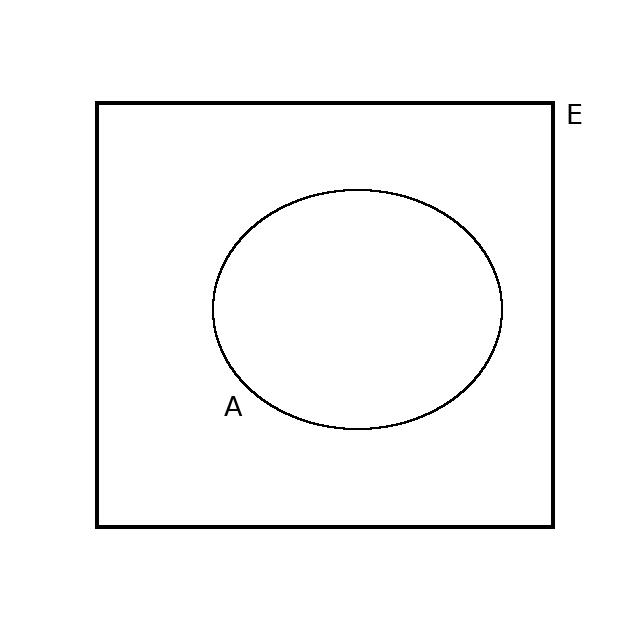
\includegraphics[width=5cm]{fig1} 
\end{center}
$$A = \{x \in E | P(x)\}$$

"$A$ est l'ensemble des $x$ de $E$ vérifiant la propriété $P$". C'est
l'ensemble solution au problème de trouver le $x$ vérifiant $P$.

Cas possible:

\begin{itemize}
    \item il y a une solution si et seulement si  $A \neq \emptyset \iff
        \exists x \in E, x \in A$

    \item il n'y a pas de solution si et seulement si $A = \emptyset \iff
        \forall x \in E, x \notin A$
\end{itemize}


\paragraph{Negation:} Propriété de $ \textrm{non}P $

$$C_{E}(A) = \bar A = \{x \in E | \ \textrm{non}P \}$$

"$\bar A$ est l'ensemble des $x$ ne vérifiant pas $P$". C'est le
\textbf{complémentaire}  de $A$ dans $E$.


\begin{center}
    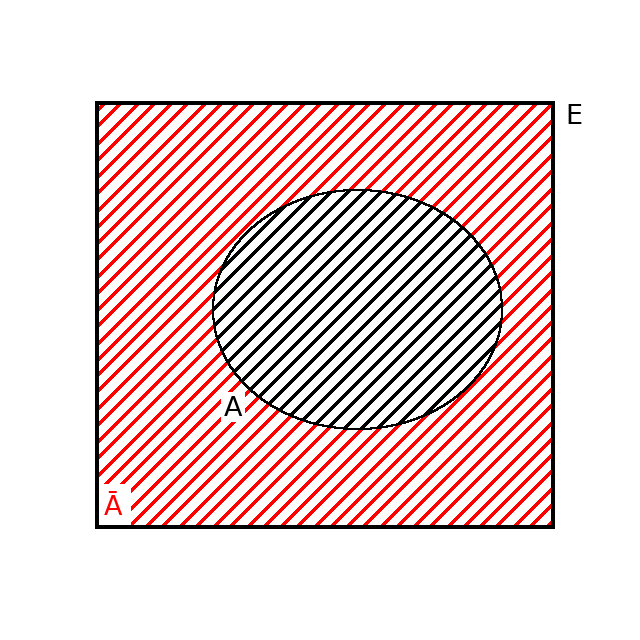
\includegraphics[width=7cm]{fig2}
\end{center}

\paragraph{Exemples}
$E = \mathbb{R}, \quad P(x) : x^{2} < 64$

$$A = \{ x \in \mathbb{R} | P(x)\} = \{x \in \mathbb{R} | x^{2} < 64 \} = ]
-8; 8 [$$

Soit $Q$ une autre propriété définie sur $E$ et $B$ l'ensemble correspondant

$$B = \{x\in E| Q(x)\}$$

\begin{center}
    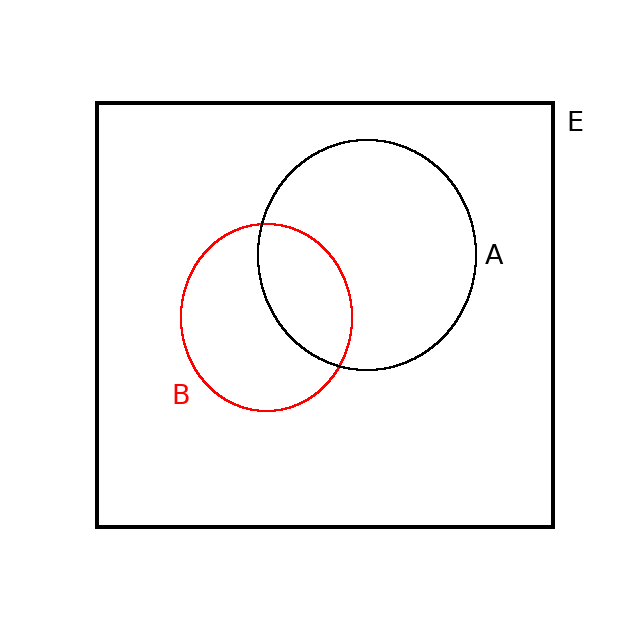
\includegraphics[width=5cm]{fig3}
\end{center}

\begin{itemize}
    \item L'ensemble des $x$ vérifiant $P$ \textbf{et} $Q$ (les deux
        conditions sont imposée) est $A \cap B$:

        $$A \cap B = \{x \in E | P(x) et Q(x)\}$$

    \item L'ensemble vérifiant $P$ \textbf{ou} $Q$ (au moins une condition est
        satisfaite) est $A \cup B$

    \item non($P$ et $Q$) est équivalent à (non$P$ ou non$Q$)

        En effet $\overline{A \cap B} = \bar A \cup \bar B$

    \item non($P$ ou $Q$) est équivalent à (non$P$ et non$Q$)

        En effet $\overline{A \cup B} = \bar A \cap \bar B$
\end{itemize}


\paragraph{Remarque}
\label{par:remarque}

Si $P$ et $Q$ sont incompatible (ne peuvent pas être vérifiés en même temps)
si $A \cap B = \emptyset$

\begin{center}
    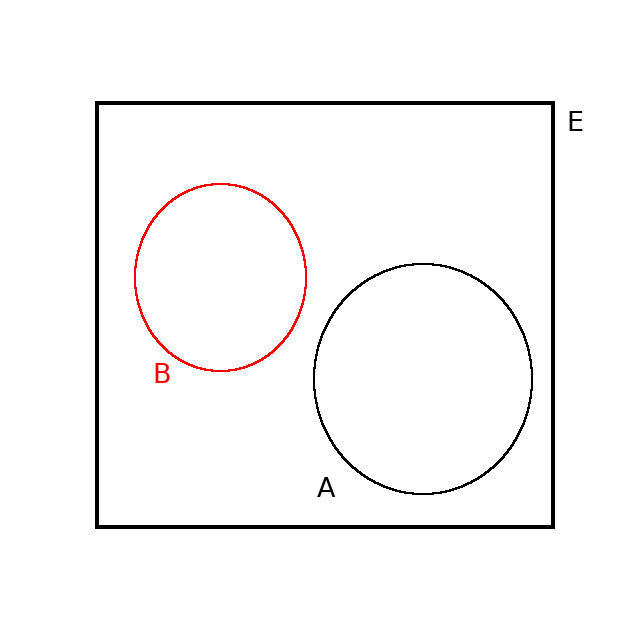
\includegraphics[width=5cm]{fig4}
\end{center}

\subsection{Propositions}
\label{sub:propositions}

Soit $P$ un propriété définie sur un référentiel $E$ et $A$ l'ensemble
correspondant.

\paragraph{Définition}
\label{par:definition}

Un proposition $T$ est une affirmation (avec un verbe!) énoncée sur les
éléments de $E$.

\begin{itemize}
    \item Proposition \textbf{simple}: sur un élément $x_{0} \in E$.
        \[
        \begin{split}
            T &: P(x_{0}) \quad "x_{0} \ \textrm{vérifie}\ P"\\
            \textrm{language ensembles}  &: T: x_{0} \in A\\
            \textrm{exemple}&: T : \sqrt{2} \ \textrm{est irrationel} 
        \end{split}
        \]

    \item Proposition \textbf{universelle}: $P$ est vérifiée par tout $x$
        \[
        \begin{split}
            T &: \forall x \in E, \quad P(x) \quad "\textrm{quelque soit}\  x, x\ \textrm{vérifie}\ P"\\
            \textrm{language ensembles}  &: T: A = E\\
            \textrm{exemple:}\ T &: \textrm{un carré est positif ou nul} 
        \end{split}
        \]

    \item Proposition \textbf{existentielle}: $P$ vérifie au moins un élément 
        \[
        \begin{split}
            T &: \exists x \in E, \quad P(x) \quad "\textrm{il existe un}\  x \ \textrm{qui vérifie}\ P"\\
            \textrm{language ensembles}  &: T: A \neq \emptyset\\
            \textrm{exemple:}\ T &: \textrm{l'equation }\ x^{2} = 2 \ \textrm{ a
            une solution} 
        \end{split}
        \]
\end{itemize}

\paragraph{Negation}
\label{par:negation}
(proposition contraire, la negation porte sur le verbe)

\begin{itemize}
    \item Proposition \textbf{simple}:
        \[
        \begin{split}
            \textrm{non} T &: \textrm{non} P(x_{0}) \quad "x_{0} \ \textrm{ne vérifie pas}\ P"\\
            \textrm{language ensembles}  &: \textrm{non} T: x_{0} \in A \ \textrm{ou} \
            x_{0} \in \bar A\\
            \textrm{exemple}&: \textrm{non} T : \sqrt{2} \ \textrm{est rationel} 
        \end{split}
        \]

    \item Proposition \textbf{universelle}: 
        \[
        \begin{split}
            \textrm{non} T &: \exists x \in E, \quad \textrm{non} P(x) \quad "\textrm{il
            existe}\  x\ \textrm{ne vérifiant pas}\ P"\\
            \textrm{language ensembles}  &: \textrm{non} T: A \neq E \ \textrm{ou
            encore}\ \bar A \neq \emptyset\\
            \textrm{exemple:}\ T &: \textrm{il existe un carré negatif} 
        \end{split}
        \]

    \item Proposition \textbf{existentielle}:
        \[
        \begin{split}
            \textrm{non} T &: \forall x \in E, \quad \textrm{non} P(x) \quad "\textrm{quelque
            soit}\  x, x \ \textrm{ne vérifie pas}\ P"\\
            \textrm{language ensembles}  &: \textrm{non} T: A = \emptyset \ \textrm{ou
            encore}\ \bar A = E\\
            \textrm{exemple:}\ T &: \textrm{l'equation }\ x^{2} = 2 \ \textrm{n'as
            pas de solution} 
        \end{split}
        \]
\end{itemize}

\subsection{Implication et equivalence}
\label{sub:implication_et_equivalence}

Soient $P$ et $Q$ deux propriétés sur $E$ et $A$ et $B$ les ensembles associés.

\begin{itemize}
    \item "$P$ implique $Q$": $P(x) \myImplies Q(x)$

        Si $x$ vérifie $P$, alors $x$ vérifie $Q$ ($P$ est plus restreint que
        $Q$)

        Tous les éléments de $A$ sont aussi éléments de $B$

        \begin{center}
            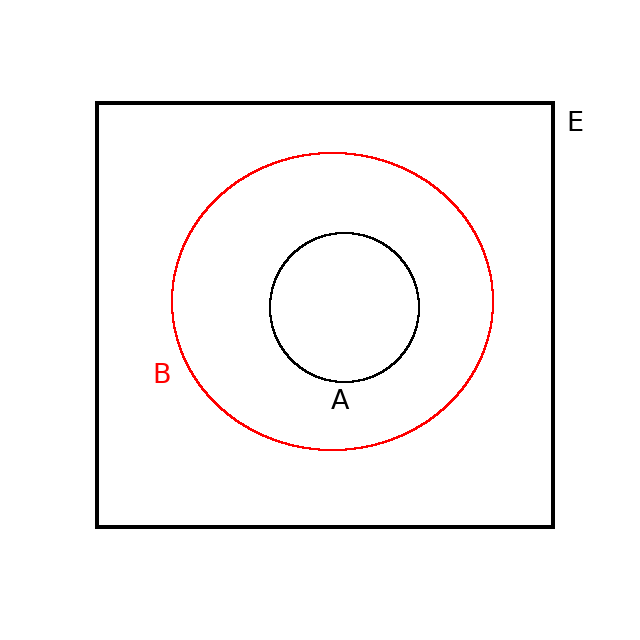
\includegraphics[width=5cm]{fig5}
        \end{center}

        Tous les éléments de $A$ sont aussi des éléments de $B$:

        $$\forall x \in A, x \in B$$

        ou

        $$\forall x \in E, \ \textrm{si}\ x \in A \ \textrm{alors}\ x \in B $$

        ou encore

        $$A \subset B$$

    \item $P$ et $Q$ sont équivalents, si et seulement si $P(x) \iff Q(x)$ si
        et seulement si $(P(x) \myImplies Q(x))$ et $(P(x) \leftarrow Q(x))$
        (\textbf{double implication}) 

        Language ensemble: $A = B$ si et seulement si $(A \subset B)$ et $(B \subset A)$
        (\textbf{double inclusion})
\end{itemize}


\paragraph{Negation de l'implication}
\label{par:negation_de_l_implication}

\[
    \begin{split}
        \textrm{non} (P \myImplies Q) & \iff \textrm{non} (\forall x \in A, x \in B)\\
        & \iff \exists x \in A, x \notin B\\
        & \iff \exists x \in E, x \in A \ \textrm{et}\ x \notin B\\
        & \iff \exists x \in E, (P(x) \ \textrm{et non}Q(x))
    \end{split}
\]


\begin{center}
    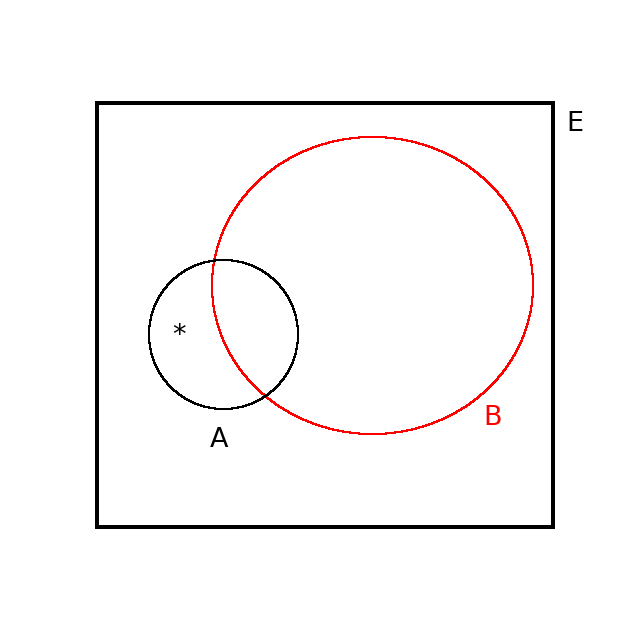
\includegraphics[width=5cm]{fig6}
\end{center}

C'est donc une proposition existentielle.

\paragraph{Exemple}
\label{par:exemple}

Tout nombre pair est multiple de 4

\begin{center}
    $T: \forall n$ pair, $n$ est multiple de 4
\end{center}

\markDate{5/03/2019}

\section{Méthode de preuve}
\label{sec:methode_de_preuve}

Une théorie mathématique se construit sur des règles que l'on donne au départ
au départ (les axiomes) et la logique.

Dans un univers de référence $E$, une proposition $T$ est soit vrai, soit
fausse (exclusif).

\paragraph{Exemples}

\begin{enumerate}
    \item La proposition

        $$T : \sqrt{2} \notin \mathbb{Q}$$

        Implicitement $E = \mathbb{R}$

    \item Une implication 

        $$T : P \implies Q$$

        \begin{itemize}
            \item $P$ est l'hypothèse: le référentiel restreint
            \item $Q$ est la conclusion.
        \end{itemize}

        \paragraph{Remarque}
        \label{par:remarque}
        
        La vérité de $Q$ n'est pas examinée "en dehors de $P$".
\end{enumerate}



\begin{center}
    \begin{minipage}{.5\textwidth}
        \resizebox{\textwidth}{!}{
            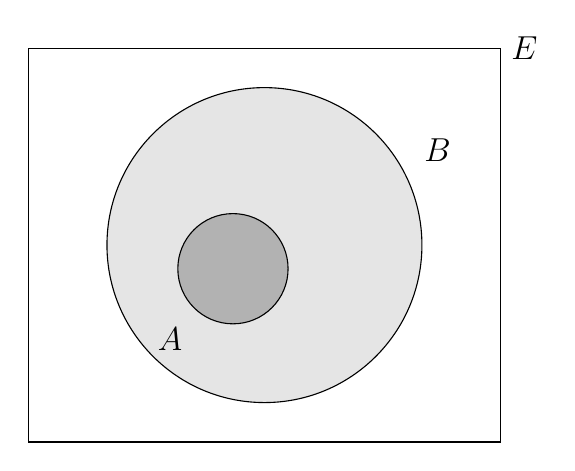
\begin{tikzpicture}
                \draw (-3cm, -2.5cm) rectangle (3cm, 2.5cm);
                \draw[fill=black!10] (0, 0) circle (2cm);
                \draw[fill=black!30] (-.4cm, -.3cm) circle (.7cm);
                \draw(-1.2cm, -1.2cm) node {$A$} ;
                \draw(2.2cm, 1.2cm) node {$B$} ;
                \draw(3.3cm, 2.5cm) node {$E$} ;
            \end{tikzpicture}
        }
    \end{minipage}
    \begin{minipage}{.49\linewidth}
        En se plaçant dans $A$  (hypothèse $P$) on est dans $B$ (conclusion $Q$)
    \end{minipage}
\end{center}


\paragraph{Exemple}

La proposition 

\begin{center}
    $T:$ si $a$ est pair, alors $a^{2}$ est pair
\end{center}

Implicitement $E$ est $\mathbb{Z}$ 

Plus simplement:

$$T: \forall a \in \mathbb{Z}, \quad a \text{ est pair } \implies a^{2} \text{ est
pair}$$

\paragraph{Remarque}

Une proposition simple $T$  peut toujours être vue comme une consequence de ce
que l'on sait sur le référentiel.

\subsection{Méthode directe}
\label{sub:methode_directe}

\paragraph{But:}
\label{par:but}
Montrer qu'une implication $$T: P \implies Q$$ est vraie (on montre que la
vérité de $Q$ en utilisant quelque part l'hypothèse $P$).

On montre $$P \implies Q$$ par une suite d'implications toutes vraies: $$P
\implies P_{1}, P_{1} \implies P_{2},\ ...\ , P_{n} \implies P_{n+1},\ ...\ ,
P_{N}  \implies Q$$

\paragraph{Exemples}

\begin{enumerate}
    \item Montrer $$T: \forall a \in \mathbb{Z}, \text{si }\underbrace{a \text{ est pair}}_{P},\text{ alors }\underbrace{a \text{ est pair}}_{Q}$$

        Soit $a \in \mathbb{Z}$ ($a$  est quelconque)

        \[
            \begin{split}
                a \text{ est pair } &\implies \exists k \in \mathbb{Z}, \quad a = 2k\\
                &\implies \exists k \in \mathbb{Z}, \quad a^{2}  = (2k)^{2} = 2\cdot\underbrace{(2k^{2})}_{k' \in\  \mathbb{Z}}\\
                &\implies \exists k' \in \mathbb{Z}, \quad a^{2} = 2\cdot k'\\
                &\implies a^{2} \text{ est pair}
            \end{split}
        \]

    \item La proposition $$T: \text{ le théorème de Pythagore}$$

        Soit un triangle rectangle

        \begin{center}
            \begin{minipage}{.5\linewidth}
                \resizebox{\textwidth}{!}{
                \begin{tikzpicture}[line cap=round,line join=round,>=triangle 45,x=1.0cm,y=1.0cm]
                    \clip(-23.130265195429633,-1.5383865869532514) rectangle (-6.540209995954007,11.001579633455757);

                    \draw [line width=0.8pt,color=ffqqqq] (-10.,0.)-- (-17.99631808831476,0.);
                    \draw [line width=0.8pt,color=ffqqqq] (-17.99631808831476,0.)-- (-10.,1.9974410208520224);
                    \draw [line width=0.8pt,color=ffqqqq] (-10.,1.9974410208520224)-- (-10.,0.);
                    \draw [line width=0.8pt] (-20.,0.)-- (-17.99631808831476,0.);
                    \draw [line width=0.8pt] (-17.99631808831476,0.)-- (-20.,8.021302129263105);
                    \draw [line width=0.8pt] (-20.,8.021302129263105)-- (-20.,0.);
                    \draw [line width=0.8pt] (-20.,10.)-- (-20.,8.021302129263105);
                    \draw [line width=0.8pt] (-20.,8.021302129263105)-- (-11.998999964758363,10.);
                    \draw [line width=0.8pt] (-11.998999964758363,10.)-- (-20.,10.);
                    \draw [line width=0.8pt] (-10.,10.)-- (-10.,1.9974410208520224);
                    \draw [line width=0.8pt] (-10.,1.9974410208520224)-- (-11.998999964758363,10.);
                    \draw [line width=0.8pt] (-11.998999964758363,10.)-- (-10.,10.);

                    \draw[color=ffqqqq] (-13.958414208471213,-0.0978910222336819) node [anchor=north]{a};
                    \draw[color=ffqqqq] (-9.786681860268282,1.1268781535665322) node [anchor=west]{b};
                    \draw[color=ffqqqq] (-13.902742882298476,1.1041928488755843) node [anchor=south]{c};

                    \draw[color=black] (-20.458041539138257,4.147047598437514) node [anchor=east] {a};
                    \draw[color=black] (-18.968833564017544,-0.0978910222336819) node[anchor=north] {b};
                    \draw[color=black] (-18.746148259326596,4.188801093067068) node {c};

                    \draw[color=black] (-15.962581950689746,10.354400466697692) node [anchor=south]{a};
                    \draw[color=black] (-20.458041539138257,9.087877796267925) node [anchor=east]{b};
                    \draw[color=black] (-15.906910624517009,8.920863817749714) node [anchor=north]{c};

                    \draw[color=black] (-9.786681860268282,6.1233796775696785) node [anchor=west]{a};
                    \draw[color=black] (-10.966080426686599,10.109029857315796) node [anchor=south]{b};
                    \draw[color=black] (-11.24339512199565,6.179051003742416) node [anchor=east]{c};
                    \end{tikzpicture}
                }
            \end{minipage}
            \begin{minipage}{.49\linewidth}
                \[
                    \begin{split}
                        (a+b)^{2} &= c^{2} + 4 \frac{ab}{2}\\
                        a^{2}  + 2ab + b^{2} &= c^{2} + 2ab\\
                        a^{2}  + b^{2}  &= c^{2} 
                    \end{split}
                \]
            \end{minipage}
        \end{center}
\end{enumerate}

\subsection{Méthode par l'absurde}
\label{sub:methode_par_l_absurde}

\paragraph{But:}

Montrer qu'une proposition $T$ est vraie.

On montre que $T$  est vraie en montrant que non$T$ est faux. non$T$  est
impossible car elle même une contradiction (absurdité).

$$T \text{ vraie } \iff [\text{ non} T \implies \text{ contradiction }]$$

\paragraph{Exemple}

$T:$ dans $\mathbb{M}_{N}(\mathbb{R})$, l'élément neutre pour le produit
matriciel est unique.

\paragraph{Preuve par l'absurde}
\label{par:preuve_par_l_absurde}

On suppose non$T$ et on montre que cela conduit à une
contradiction. $$\text{non}T: \text{ dans } \mathbb{M}_{N}(\mathbb{R}) \text{ il
existe plus d'un élément neutre pour le produit matriciel} $$

Notons $ I_{n} $ et $ N_{n} $ des éléments neutre, avec $ I_{n} \ne N_{n} $.

Alors $$I_{n} = I_{n} \cdot N_{n} = N_{n}$$ D'où la contradiction avec $$I_{n}
\ne N_{n}$$

\paragraph{Remarque}

Cas d'une proposition universelle sur l'ensemble $E$ $$T: \forall x \in E,
\quad x \text{ vérifie } P$$ Par l'absurde, on doit montrer l'implication $$[\
    \exists x \in E,\ x \text{ vérifie non}P\ ] \implies \text{ contradiction
    } $$ (mise en défaut de l'existence d'un contre-exemple)

Cela est équivalent à dire $$\forall x \in E, \ [\ x \text{ vérifie non}P
    \implies \text{ contradiction } ] $$ (aucun élément n'est un contre-exemple)

\paragraph{Rappel}
\label{par:rappel}

\Warning Si $T$ est une implication $P \implies Q$, sa négation non$T$ n'est
par une proposition universelle.

\begin{center}
    \begin{minipage}{.5\textwidth}
        \resizebox{\textwidth}{!}{
            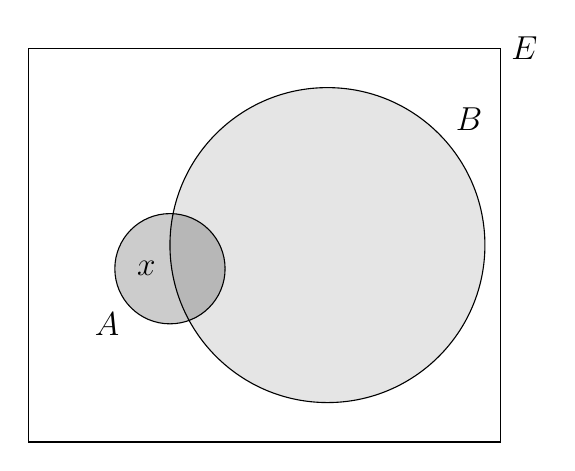
\begin{tikzpicture}
                \draw (-3cm, -2.5cm) rectangle (3cm, 2.5cm);
                \draw[fill=black!10] (.8cm, 0) circle (2cm);
                \draw[fill=black, fill opacity = .2] (-1.2cm, -.3cm) circle (.7cm);

                \draw(-1.5cm, -.3cm) node {$x$} ;
                \draw(-2cm, -1cm) node {$A$} ;
                \draw(2.6cm, 1.6cm) node {$B$} ;
                \draw(3.3cm, 2.5cm) node {$E$} ;
            \end{tikzpicture}
        }
    \end{minipage}
    \begin{minipage}{.49\linewidth}
        \[
            \begin{split}
                T&: \forall x \in E, \quad P(x) \implies Q(x)\\
                \text{ non}T &: \exists x \in E, \quad P(x) \text{ et }  \text{ non}Q(x)\\
            \end{split}
        \]
    \end{minipage}
\end{center}

\subsection{Méthode indirecte ou contraposée}
\label{sub:methode_indirecte_ou_contraposee}

\paragraph{But}

Montrer qu'une implication $$T: P \implies Q$$ est vraie.

\paragraph{Définition}

Soit la proposition $$T: P \implies Q$$ la proposition $$C: \text{ non}Q
\implies \text{ non}P$$ est la contraposée de $T$.

\pagebreak

$C$ et $T$ sont équivalent. En effet $$T: A \subset B \quad \quad \quad \quad
\quad C: \bar B \subset \bar A$$

\begin{center}
    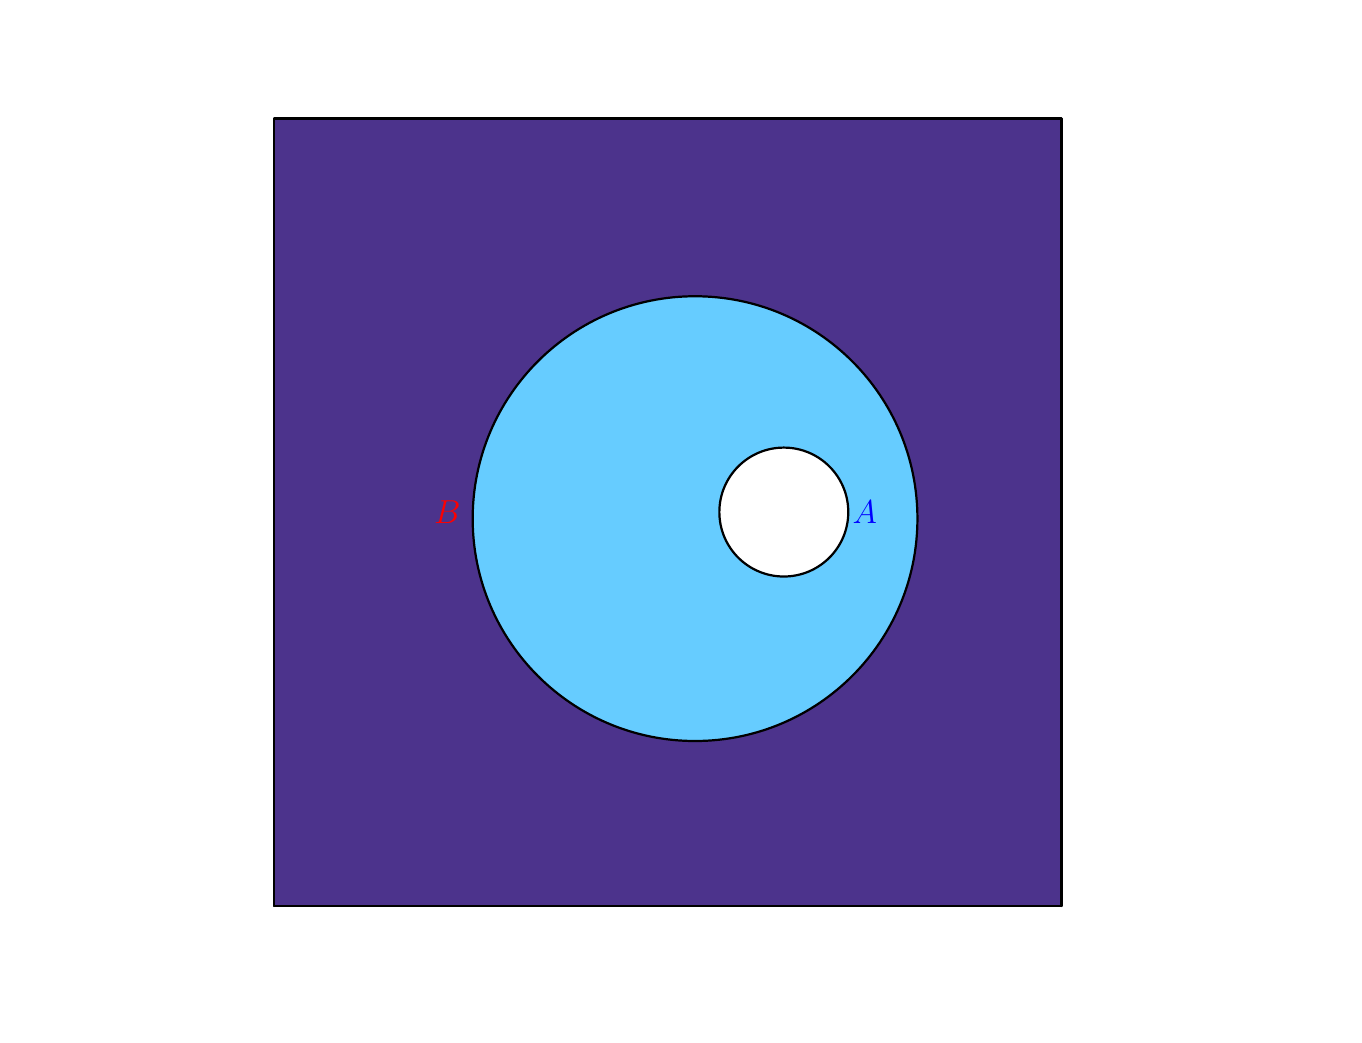
\begin{tikzpicture}[line cap=round,line join=round,>=triangle 45,x=1.0cm,y=1.0cm]
    \clip(-23.130265195429637,-1.3852904399782258) rectangle (-6.540209995954008,11.154675780430786);
    \fill[line width=0.4pt,color=ttqqqq] (-20.,0.) -- (-10.,0.) -- (-10.,10.) -- (-20.,10.) -- cycle;
    \fill[line width=0.4pt,color=ffwwzz,fill=ffwwzz,fill opacity=0.5] (-20.,0.) -- (-10.,0.) -- (-10.,10.) -- (-20.,10.) -- cycle;
    \fill[line width=0.4pt,color=qqttcc,fill=qqttcc,fill opacity=0.5] (-20.,0.) -- (-10.,0.) -- (-10.,10.) -- (-20.,10.) -- cycle;
    \draw [line width=0.8pt,color=black,fill=wwccff,fill opacity=1.0] (-14.654305785630436,4.919487249084238) circle (2.82422261828165cm);
    \draw [line width=0.8pt,color=black,fill=ffffff,fill opacity=1.0] (-13.526961430632502,5.002994238343346) circle (0.8186714118808677cm);
    \draw [line width=0.8pt] (-20.,0.)-- (-10.,0.);
    \draw [line width=0.8pt] (-10.,0.)-- (-10.,10.);
    \draw [line width=0.8pt] (-10.,10.)-- (-20.,10.);
    \draw [line width=0.8pt] (-20.,10.)-- (-20.,0.);
    \begin{scriptsize}
    \draw[color=ffqqqq] (-17.8,5) node {$B$};
    \draw[color=qqqqff] (-12.5,5) node {$A$};
    \end{scriptsize}
    \end{tikzpicture}
\end{center}


\paragraph{Exemple}

Démontrer $$T: \forall a \in \mathbb{Z}, \text{ si } a^{2} \text{ est pair}
, \text{ alors } a \text{ est pair } $$

\paragraph{Remarque}

méthode directe, pas facile!

Preuve par contraposée: $$C: \forall a \in \mathbb{Z}, \text{ si }
\underbrace{a \text{ est impair}}_{\text{ non}Q}, \text{ alors } \underbrace{a^{2} \text{ est impair}}_{\text{ non}P}$$

En effet (directement)

\[
    \begin{split}
        a \text{ est impair } &\implies \exists k \in \mathbb{Z}, \quad a = 2k
        + 1\\
        &\implies \exists k \in \mathbb{Z}, \quad a^{2} = (2k+1)^{2} = 4k^{2}
        + 4k + 1 = 2\cdot\underbrace{(2k^{2} + 2k)}_{k' \in \mathbb{Z}} + 1\\
        &\implies \exists k' \in \mathbb{Z}, \quad a^{2} = 2 k' + 1\\
        &\implies a ^{2} \text{ est impair }
    \end{split}
\]

Donc $C$ est vraie et donc $T$ est vraie.


\subsection{Méthode par induction (ou par récurrence)}
\label{sub:methode_par_induction_ou_par_recurrence_}

\paragraph{But}

montrer qu'une proposition $T(n)$ dépendant d'un entier positif $n$ est vraie
à partir d'un certain rang $n_{0}$: $$\exists n_{0} \in \mathbb{N}^{*}, \quad
[\ \forall n \geq n_{0}, T(n) \text{ vraie } ]$$

\paragraph{Théorème d'induction}
\label{par:theoreme_d_induction}

Une proposition $T(n)$ est vraie $\forall n \geq n_{0}$ si et seulement si 

\begin{enumerate}
    \item $\exists n_{0} \in \mathbb{N}^{*} \tq T(n_{0})$ vraie.
    \item $\forall n \geq n_{0} \ [\ T(n) \text{ vraie }  \implies T(n+1) \text{ vraie } ]$ 
\end{enumerate}

\paragraph{Exemple}

Soit le nombre suivant (définition)

\[
    \begin{split}
    S_{n} &= 1 \cdot 1! + 2 \cdot 2! + 3 \cdot 3! + ... + n\cdot n !\\
    &= \sum^{n}_{k=1} k\cdot k! \quad \quad (n \in \mathbb{N}^{*})
    \end{split}
\]

Démontrer la proposition suivant $$\forall n \in \mathbb{N}^{*}, \quad S_{n} =
(n+1)! -1$$

Notons $$T(n): S_{n} = (n+1)! -1$$

\begin{enumerate}
    \item Prenons $n_{0} = 1$, vérifions $T(n_{0})$ 

        \begin{enumerate}
            \item Calculons $S_{n_{0}} = S_{1} = 1 \cdot 1 ! = 1$  (définition)
            \item D'autres part $(n_{0} + 1)! -1 = 2! -1 = 1 \quad \checkmark.$
        \end{enumerate}
    \item  A montrer $$\forall n \geq n_{0} = 1:$$

        \[
            \begin{split}
                \text{ Hypothèse } \quad \quad \quad \quad \quad T(n) : S_{n} &= (n+1) ! - 1\\
                \text{ Conclusion } \quad \quad \quad T(n+1) : S_{n} &= (n+2) ! - 1\\
            \end{split}
        \]

        En effet
        \[
            \begin{split}
                S_{n+1} &= 1\cdot 1 ! + 2 \cdot 2 ! + ... + n\cdot n! + (n+1)\cdot(n+1)!\\
                &= S_{n} + (n+1)\cdot (n+1)!\\
                &= (n+1)! - 1 + (n+1)\cdot(n+1) \\
                &= (1+n+1)\cdot(n+1)!-1\\
                &= (n+2)! -1
            \end{split}
        \]
        \cqfd
\end{enumerate}


\subsection{Le contre-exemple}
\label{sub:le_conte_exemple}

\paragraph{But}

Montrer qu'une proposition universelle est fausse.

Soit une proposition universelle $$T: \forall x \in E E, \quad x \text{ vérifie } P$$

$T$ est fausse si et seulement si non$T$ est vraie. On montera donc que la
proposition existentielle non$T$ est vraie. $$ \text{ non}T: \exists x \in E,
x \text{ vérifie non}P $$ On montre avec l'existence d'un $x$ ne vérifiant pas
P: un contre-exemple.

\paragraph{Exemple}

$$T : \text{ tous les nombres premiers sont impairs }$$

$T$ est fausse, donnons un contre-exemple selon la négation de $T$ .

$$ \text{ non}T: \text{ il existe un nombre premier qui est pair }$$

Par exemple $n=2$ (\textbf{remarque}: c'est le seul)

Formellement

\[
    \begin{split}
        T:& \forall a \in \mathbb{N}^{*}, \quad a \text{ premier } \implies a \text{ impair }\\
        \text{ non}T:& \exists a \in \mathbb{N}^{*}, \quad a \text{ premier et } a \text{ pair }\\
    \end{split}
\]


\end{document}
